% !TeX spellcheck = cs_CZ
{\tikzset{external/prefix={tikz/FYZII/}}
 \tikzset{external/figure name/.add={ch24_}{}}
%---------------------------------------------------------------------------------------------------
% file fey2ch24.tex
%---------------------------------------------------------------------------------------------------
%=========================== Kapitola Vlnovody =====================================================
\chapter{Vlnovody}\label{fyz:IIchaXXIV}
\minitoc
  \section{Přenosové vedení}\label{fyz:IIchaXXIVsecI}
  \section{Obdélníkový vlnovod}\label{fyz:IIchaXXIVsecII}
  \section{Mezní frekvence}\label{fyz:IIchaXXIVsecIII}
  \section{Rychlost šíření vln ve vlnovodu}\label{fyz:IIchaXXIVsecIV}
  \section{Detekování vedených vln}\label{fyz:IIchaXXIVsecV}
  \section{Spojování vlnovodů}\label{fyz:IIchaXXIVsecVI}
  \section{Mody vlnovodů}\label{fyz:IIchaXXIVsecVII}
  \section{Jiný pohled na vlnovody}\label{fyz:IIchaXXIVsecVIII}
  \section{Příklady a cvičení}\label{fyz:IIchaXXIVsecIX}

    \begin{figure}[ht!] %\ref{fyz_fig559}
      \centering
      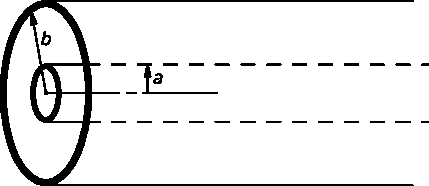
\includegraphics[width=0.7\linewidth]{fyz_fig559.pdf}
      \caption{
               (\cite[s.~707]{Feynman02})}
      \label{fyz_fig559}
    \end{figure}

    \begin{figure}[ht!] %\ref{fyz_fig560}
      \centering
      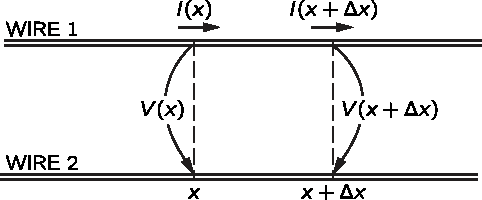
\includegraphics[width=0.7\linewidth]{fyz_fig560.pdf}
      \caption{
               (\cite[s.~707]{Feynman02})}
      \label{fyz_fig560}
    \end{figure}

    \begin{figure}[ht!] %\ref{fyz_fig561}
      \centering
      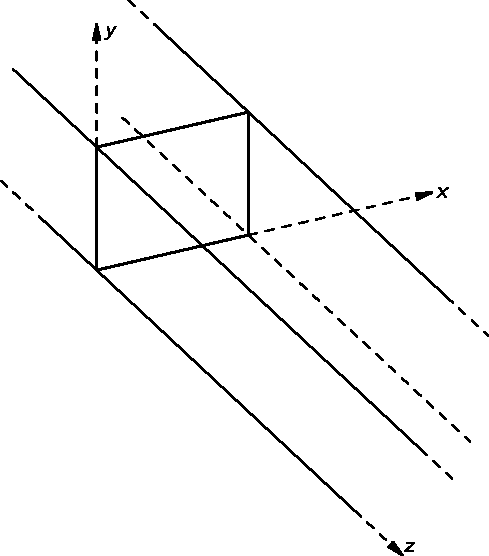
\includegraphics[width=0.7\linewidth]{fyz_fig561.pdf}
      \caption{
               (\cite[s.~707]{Feynman02})}
      \label{fyz_fig561}
    \end{figure}

    \begin{figure}[ht!] %\ref{fyz_fig562}
      \centering
      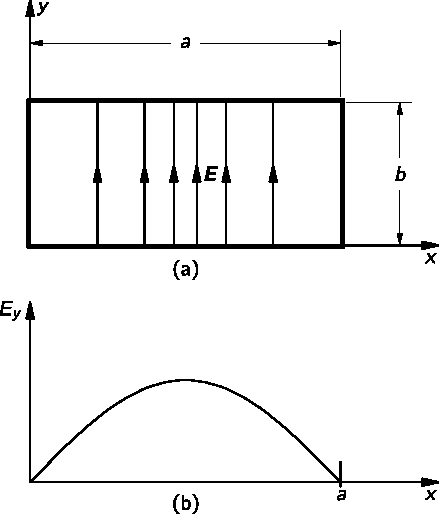
\includegraphics[width=0.7\linewidth]{fyz_fig562.pdf}
      \caption{
               (\cite[s.~707]{Feynman02})}
      \label{fyz_fig562}
    \end{figure}

    \begin{figure}[ht!] %\ref{fyz_fig563}
      \centering
      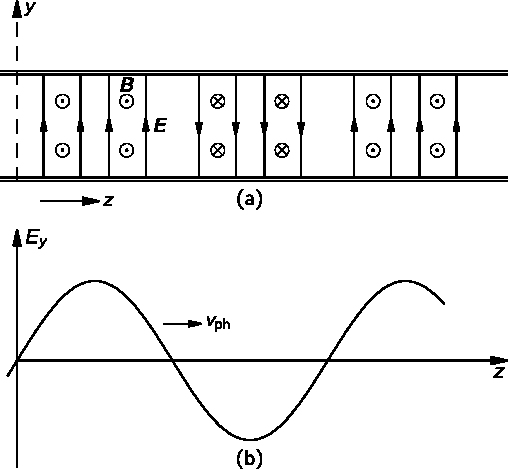
\includegraphics[width=0.7\linewidth]{fyz_fig563.pdf}
      \caption{
               (\cite[s.~707]{Feynman02})}
      \label{fyz_fig563}
    \end{figure}

    \begin{figure}[ht!] %\ref{fyz_fig564}
      \centering
      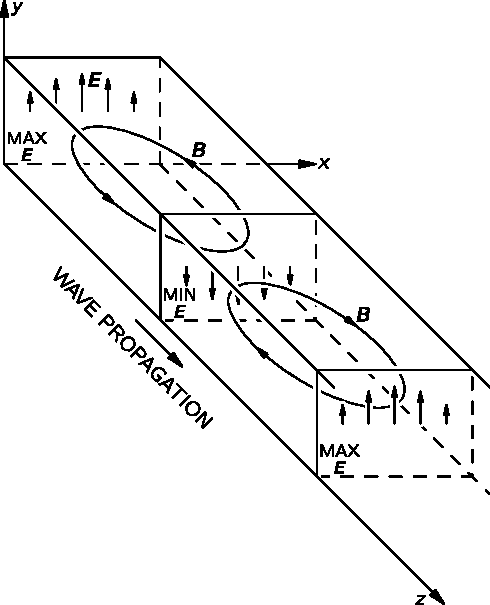
\includegraphics[width=0.7\linewidth]{fyz_fig564.pdf}
      \caption{
               (\cite[s.~707]{Feynman02})}
      \label{fyz_fig564}
    \end{figure}

    \begin{figure}[ht!] %\ref{fyz_fig565}
      \centering
      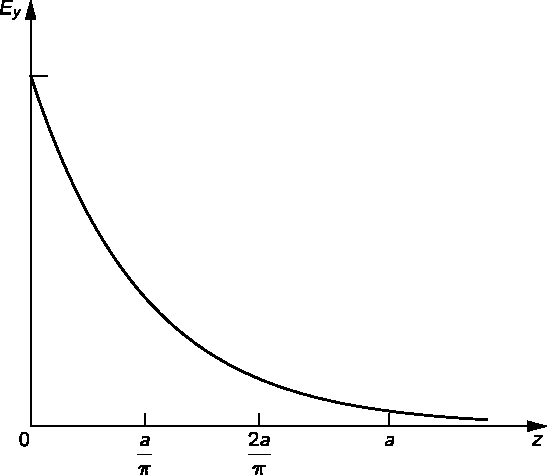
\includegraphics[width=0.7\linewidth]{fyz_fig565.pdf}
      \caption{
               (\cite[s.~707]{Feynman02})}
      \label{fyz_fig565}
    \end{figure}

    \begin{figure}[ht!] %\ref{fyz_fig566}
      \centering
      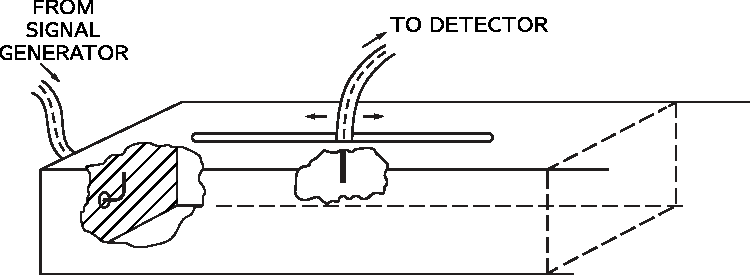
\includegraphics[width=0.7\linewidth]{fyz_fig566.pdf}
      \caption{
               (\cite[s.~707]{Feynman02})}
      \label{fyz_fig566}
    \end{figure}

    \begin{figure}[ht!] %\ref{fyz_fig567}
      \centering
      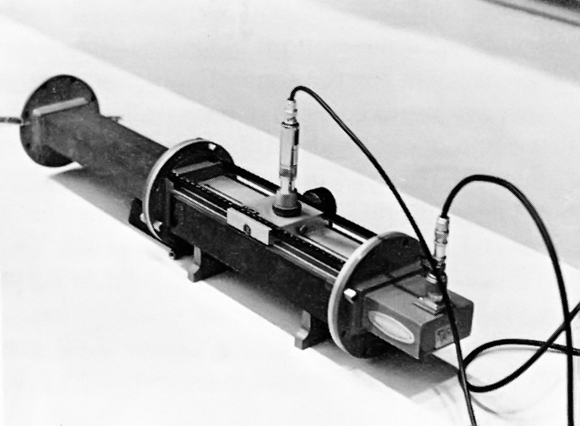
\includegraphics[width=0.7\linewidth]{fyz_fig567.jpg}
      \caption{
               (\cite[s.~707]{Feynman02})}
      \label{fyz_fig567}
    \end{figure}

    \begin{figure}[ht!] %\ref{fyz_fig568}
      \centering
      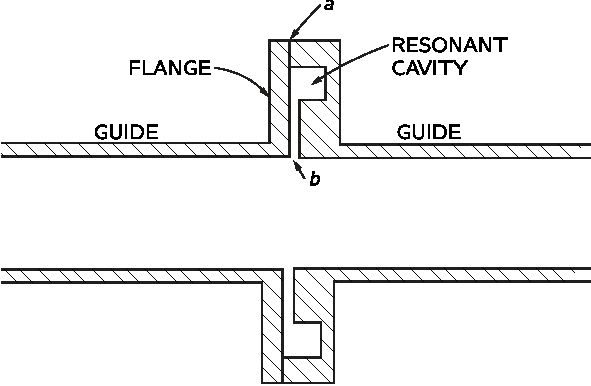
\includegraphics[width=0.7\linewidth]{fyz_fig568.pdf}
      \caption{
               (\cite[s.~707]{Feynman02})}
      \label{fyz_fig568}
    \end{figure}

    \begin{figure}[ht!] %\ref{fyz_fig569}
      \centering
      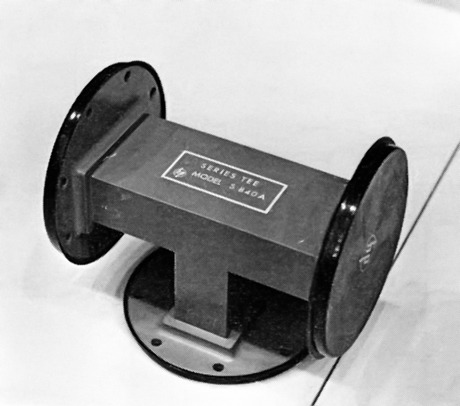
\includegraphics[width=0.7\linewidth]{fyz_fig569.jpg}
      \caption{
               (\cite[s.~707]{Feynman02})}
      \label{fyz_fig569}
    \end{figure}

    \begin{figure}[ht!] %\ref{fyz_fig570}
      \centering
      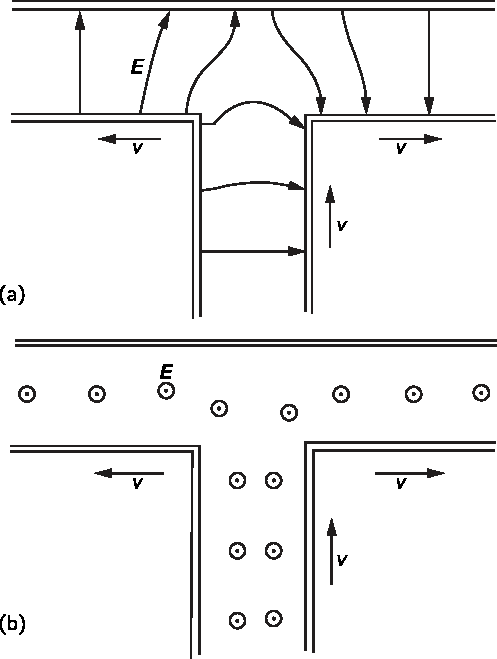
\includegraphics[width=0.7\linewidth]{fyz_fig570.pdf}
      \caption{
               (\cite[s.~707]{Feynman02})}
      \label{fyz_fig570}
    \end{figure}

    \begin{figure}[ht!] %\ref{fyz_fig571}
      \centering
      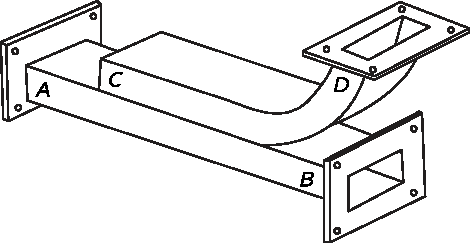
\includegraphics[width=0.7\linewidth]{fyz_fig571.pdf}
      \caption{
               (\cite[s.~707]{Feynman02})}
      \label{fyz_fig571}
    \end{figure}

} %tikzset
%---------------------------------------------------------------------------------------------------
\printbibliography[title={Seznam literatury},heading=subbibliography]
\addcontentsline{toc}{section}{Seznam literatury}